\chapter{Method}
\label{chap:method}
This chapter presents the research method used in this thesis. Firstly, the research motivation is presented, followed by the research questions defined for this thesis. Finally, the research method and design is explained.

\section{Research Motivation}

Existing solutions are slow.
A total of X new contrats are deployed  each day on the Ethereum network. Witth tthe speedup of the upgraded ethereum network,  this is likely to result in an utterly spike  in deployed contracts. Existing solutions are scarse. Further, the few ones available are based on symbolic analysis.  Tthis is a very slow approach. It is therefore not possible to process all new contractts due to time resttrictions. An natural approach for combatting this is by leveraging deep learning techniques.





\section{Research Questions}
\label{sec:research-questions}
The research questions addressed in this thesis are:
\begin{enumerate}[label=RQ\arabic*., leftmargin=1.5cm]
    \item Officia magna irure ut occaecat cupidatat non sunt sunt.
\end{enumerate}

\section{Research Method and Design}
\label{sec:research-method-and-design}

\begin{figure}[htp]
    \centering
    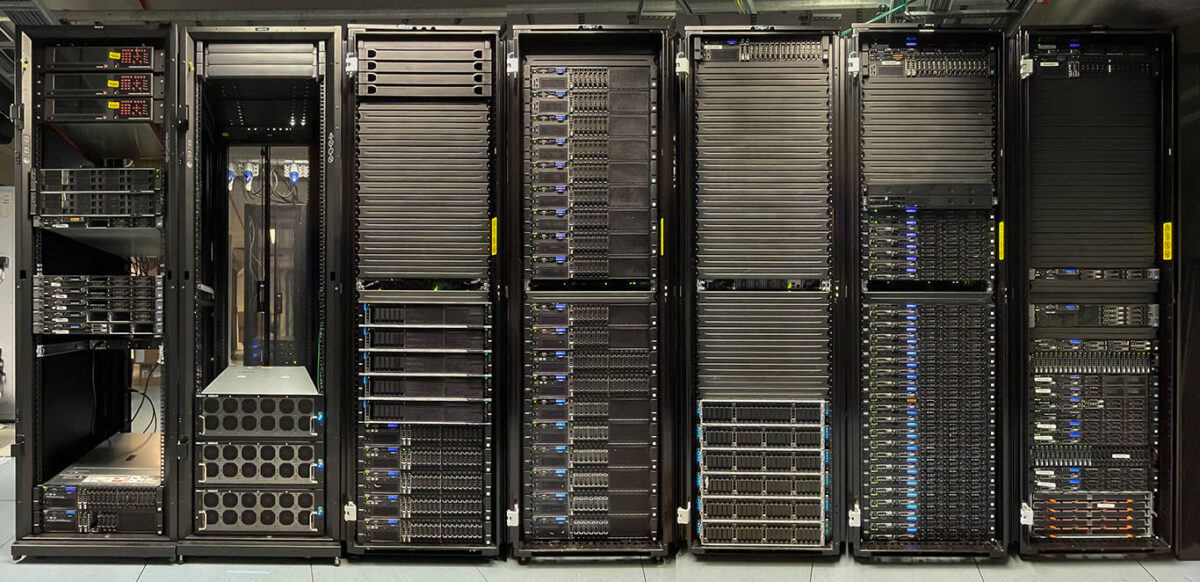
\includegraphics[width=\textwidth]{figures/idun.jpeg}
    \caption{Image of IDUN todo: add ref \url{https://www.hpc.ntnu.no/idun/}}
    \label{fig:flowchart}
\end{figure}

\section{Tools and Libraries}
\label{sec:tools-and-libraries}

\section{Hardware resources}
\label{sec:hardware-resources}

\subsection{IDUN High Performance Computing Platform}
\label{sec:idun-high-performance-computing-platform}